\chapter{Design Overview}

\section{General Design}

My app design is envisioned as a tab-based application, ensuring straightforward navigation and user-friendly interaction. This approach allows users to easily access different sections of the app, keeping the user experience organized and intuitive.

I decided to place a strong emphasis on minimalistic design principles to create an uncluttered and efficient interface. By stripping away unnecessary elements and focusing on essential functionalities, the app becomes user-centric and easy to use, enhancing the overall user experience.

For the color scheme, I drew inspiration from the concept of cool colors. Cool colors, with their calming and relaxing properties, are chosen to evoke a sense of tranquility and ease within the app, ensuring users feel at ease and comfortable during their interaction with the platform \cite{Bilucaglia}.

\begin{figure}[H]
    \centering
    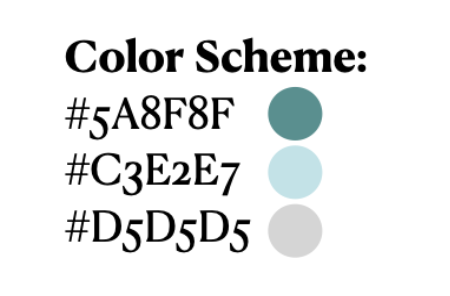
\includegraphics[width=0.2\linewidth]{thesis//chapters//images/colorScheme.png}
    \caption{Color Scheme}
    \label{fig:color-scheme}
\end{figure}

In addition, I aim to provide a design that is inclusive and accessible to all users. To achieve this, I carefully considered contrast and color choices, making sure they were tested against colorblind scales to ensure that the content is easily distinguishable and readable by a wide range of individuals.

To add a friendly and inviting touch to the app, I incorporated images and graphics that resonate with a warm and approachable feel. These images are thoughtfully chosen to create a connection with users and enhance their engagement with the app, contributing to a positive and enjoyable user experience.

In the following sections, you will see my initial prototype designs.

\section{Onboarding View}

The onboarding view consists of screens designed to introduce users to the app's key features and benefits. This view is essential for guiding new users and helping them get acquainted with the platform. The screens are simplistic and visually appealing, setting a positive tone for the user's journey.

The Set Up form asks the user to input key information, such as their name, birthdate, and allergens, and asks the user if they will allow the application to share data with Apple Health. This is a crucial step in the onboarding process, as without allowing access, the user will not have access to key insights and a tailored app experience.

\begin{figure}[H]
    \centering
    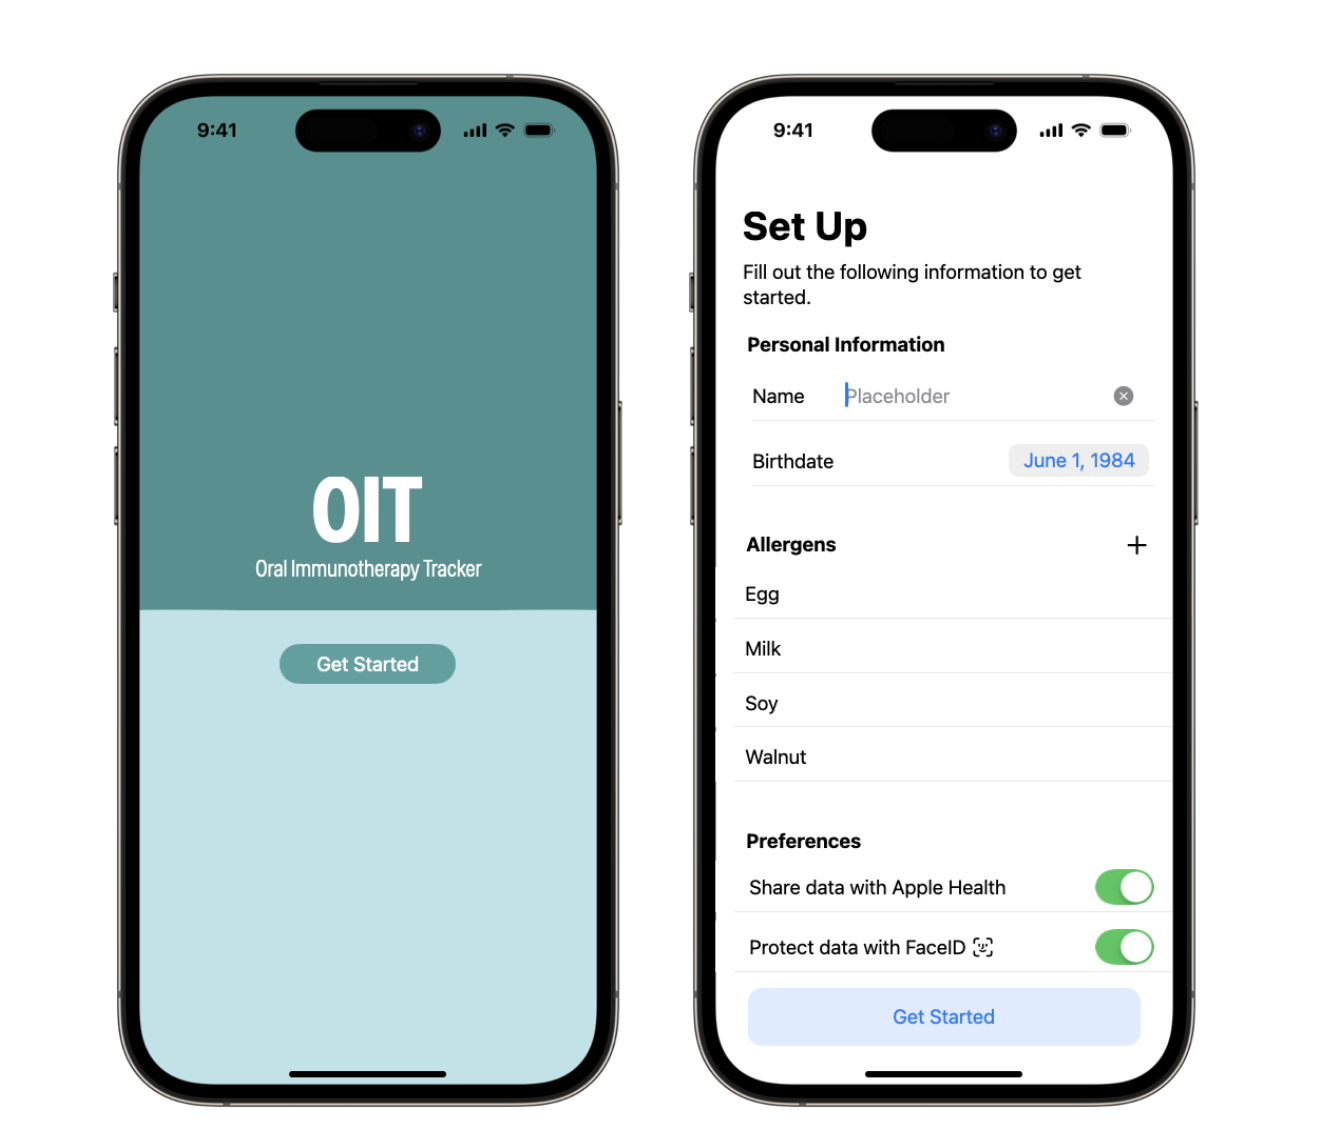
\includegraphics[width=0.7\linewidth]{thesis//chapters//images/onboarding-screens.png}
    \caption{Onboarding Screens}
    \label{fig:onboarding-screens}
\end{figure}

\section{Today Tab}

The Today Tab serves as the core of the app, where users view and log dose and symptom information for the selected date. The design prioritizes clarity and easy navigation, ensuring that users can quickly find the information they need. A sliding weekly calendar view allows the user to select a date, or the month button in the top right corner allows the user to switch to a monthly view. 

\begin{figure}[H]
    \centering
    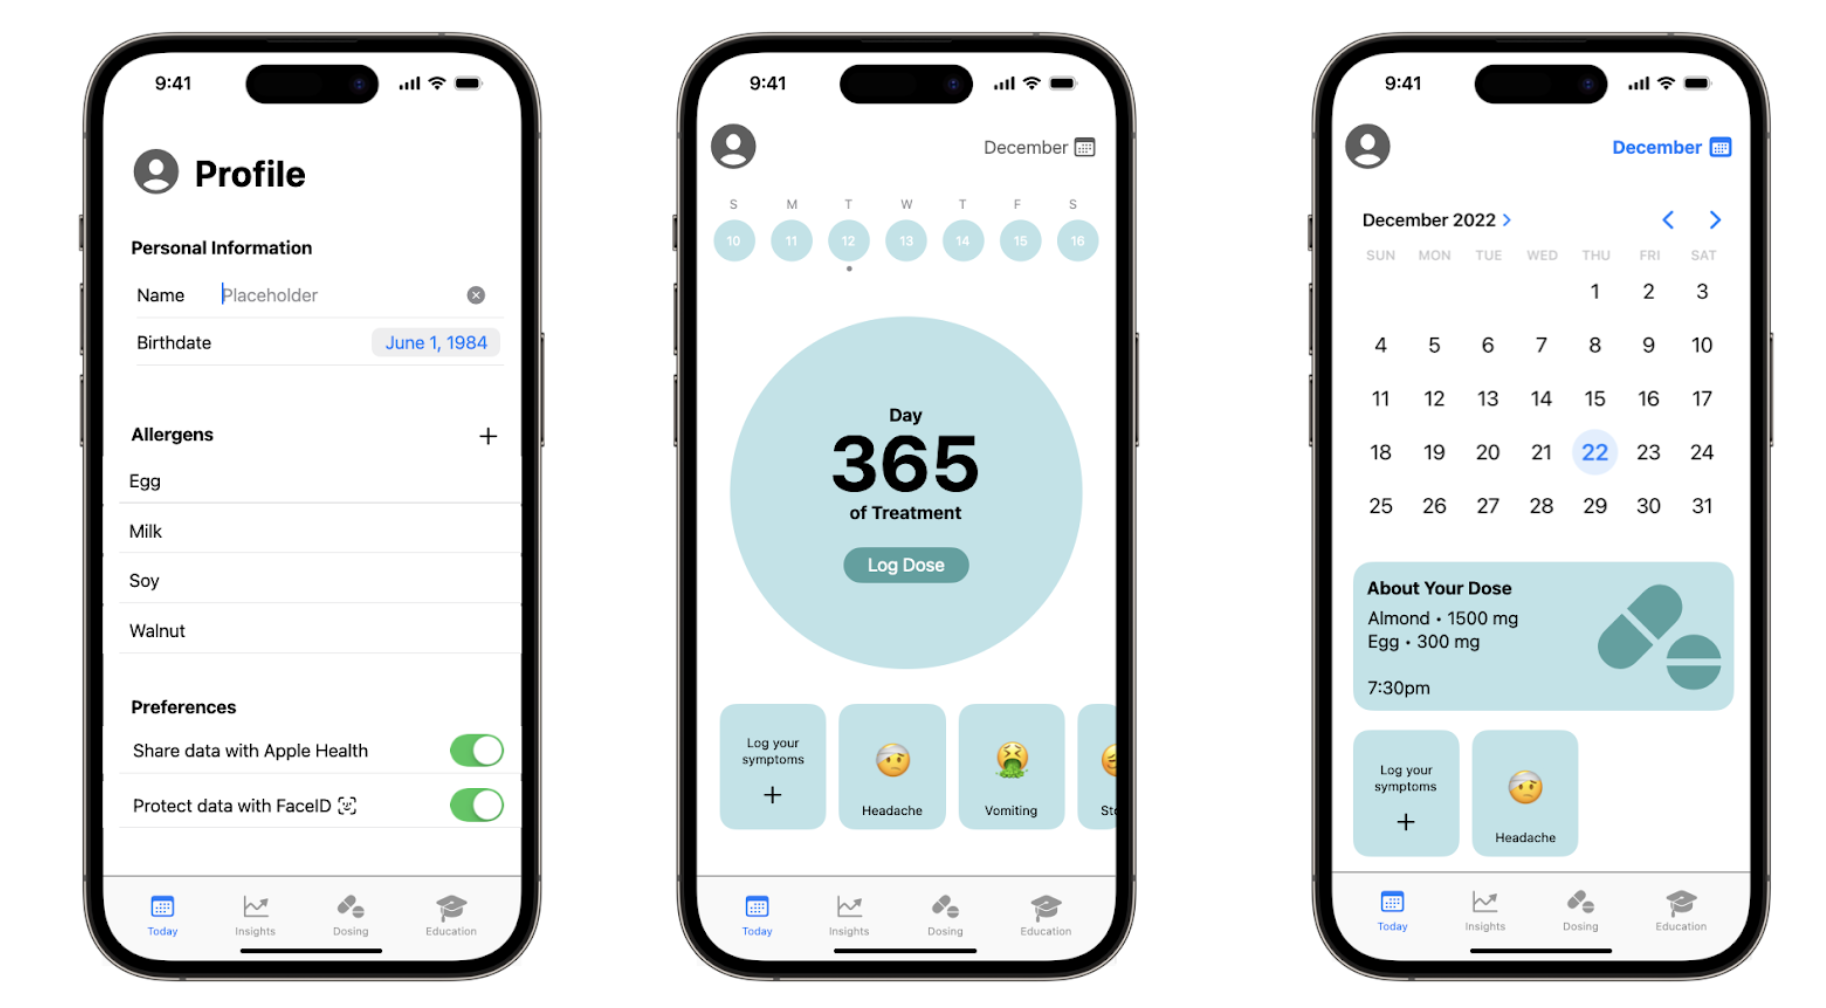
\includegraphics[width=1\linewidth]{thesis//chapters//images/todayTabScreens.png}
    \caption{Today Tab Screens}
    \label{fig:today-tab-screens}
\end{figure}

\section{Dose and Symptom Pop-Ups}

The dose and symptom pop-ups are opened when the user goes to log a dose or symptom in the Today tab. These pop-ups are designed to be user-friendly, with helpful graphics, and to make it take minimal time to log a dose or symptom.

\begin{figure}[H]
    \centering
    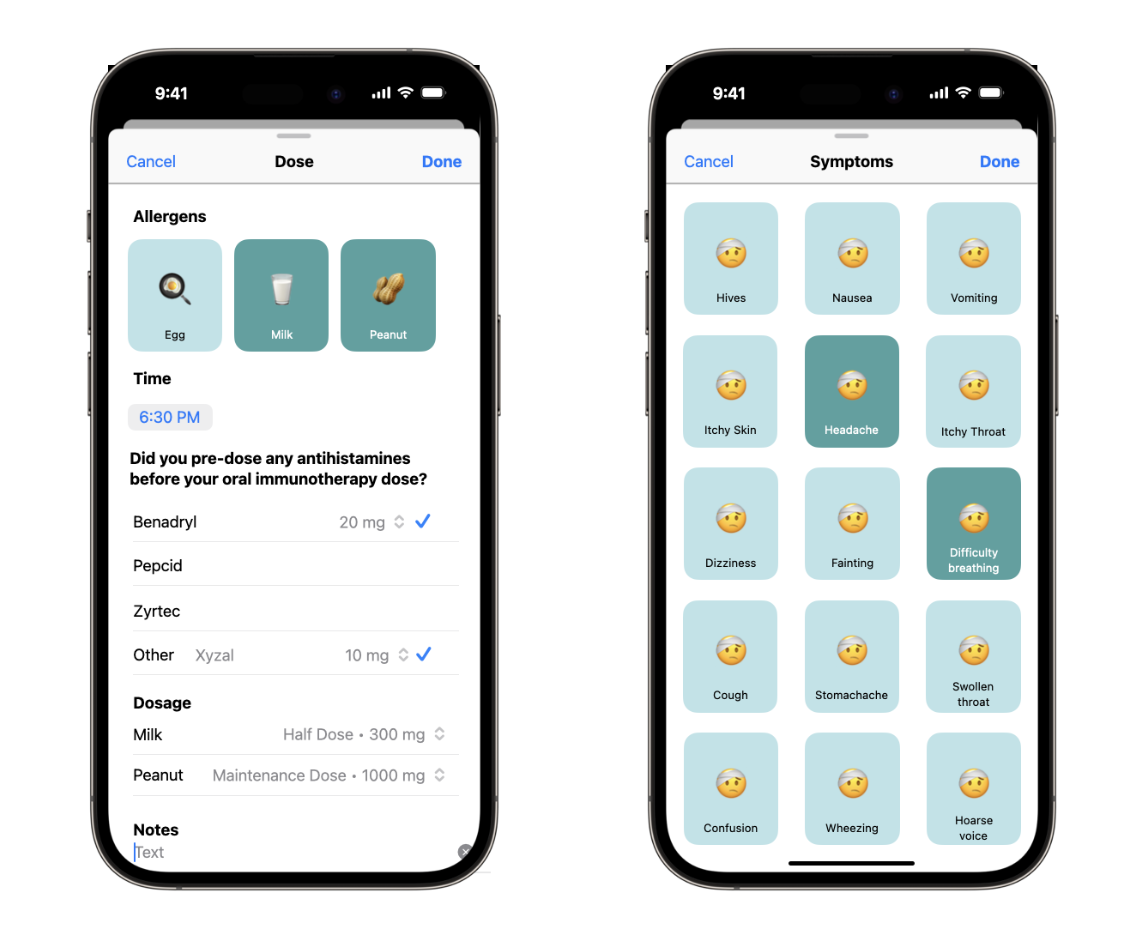
\includegraphics[width=0.7\linewidth]{thesis//chapters//images/doseAndSymptomPopUps.png}
    \caption{Dose and Symptoms Pop-Ups}
    \label{fig:dose-and-symptom-pop-ups}
\end{figure}

\section{Insights Tab}

\begin{figure}[H]
    \centering
    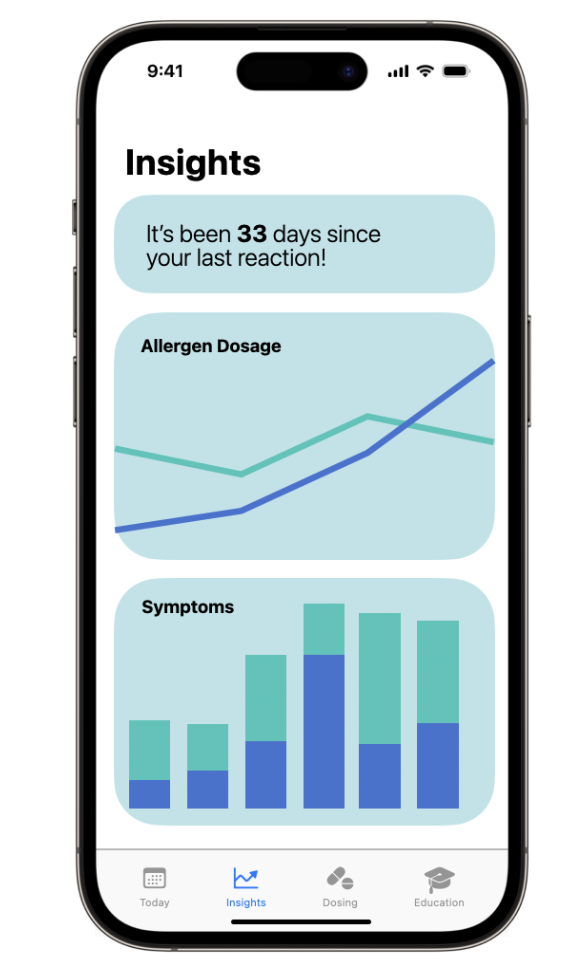
\includegraphics[width=0.3\linewidth]{thesis//chapters//images/insightsTab.png}
    \caption{Insights Tab}
    \label{fig:insights-tab}
\end{figure}

\section{Dosing Tab}

The dosing tab

\begin{figure}[H]
    \centering
    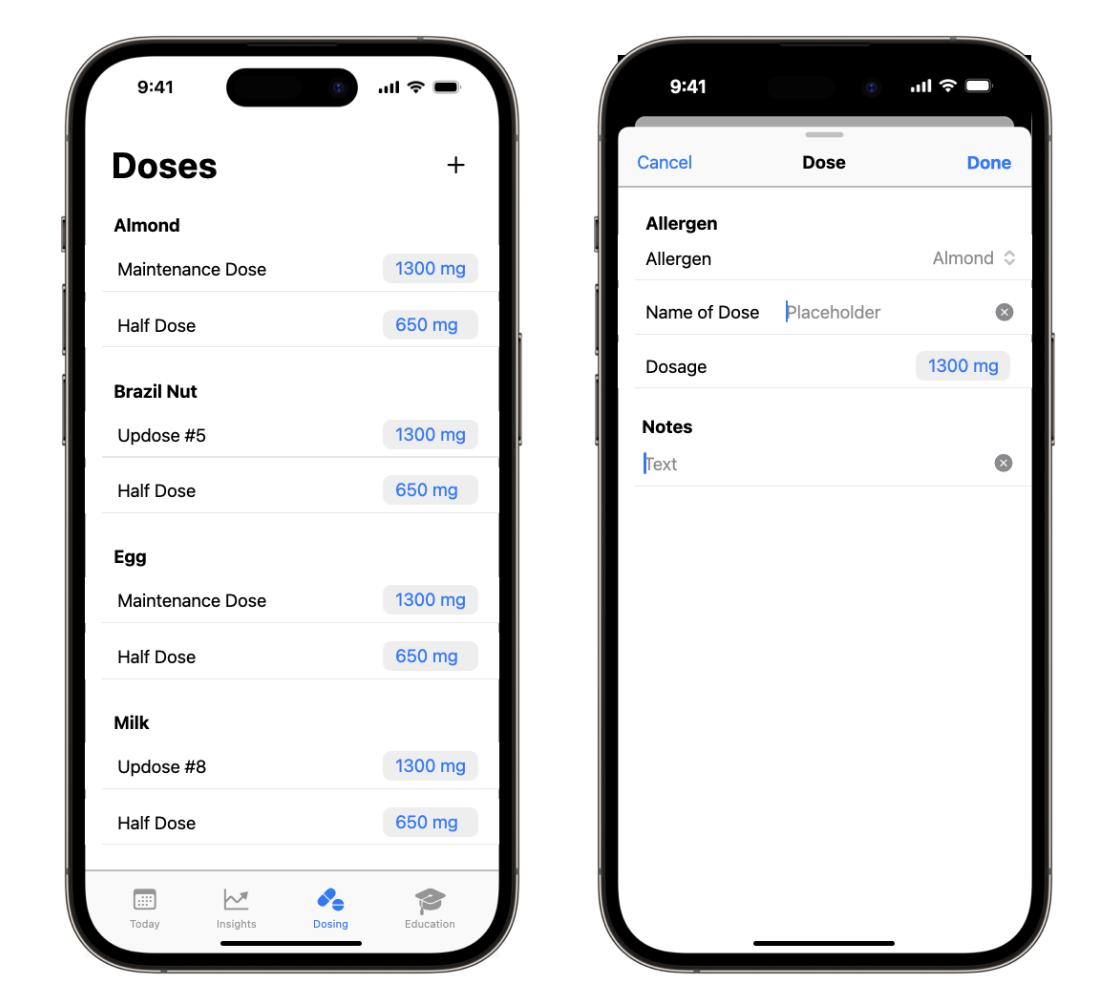
\includegraphics[width=0.7\linewidth]{thesis//chapters//images/dosingTabScreens.png}
    \caption{Dosing Tab Screens}
    \label{fig:dosing-tab}
\end{figure}

\section{Education Tab}

\begin{figure}[H]
    \centering
    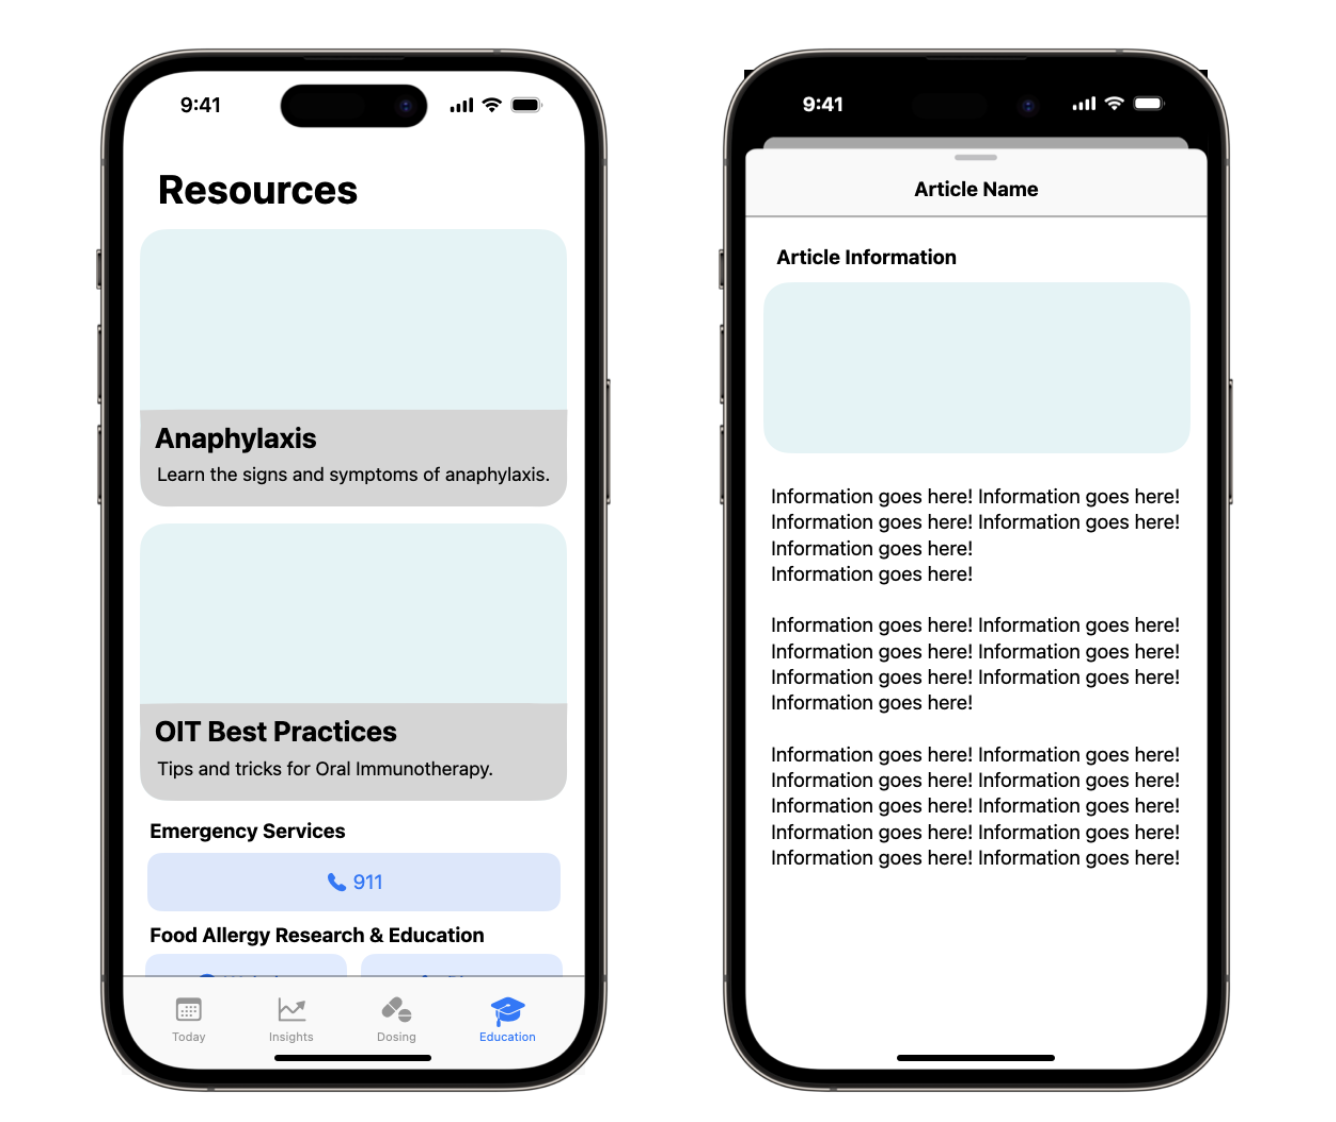
\includegraphics[width=0.7\linewidth]{thesis//chapters//images/education-tab-screens.png}
    \caption{Education Tab Screens}
    \label{fig:education-tab}
\end{figure}

